\documentclass[12pt]{article}
\usepackage{graphicx}

%%% margins 
\textheight 23.4cm
\textwidth 14.65cm
\oddsidemargin 0.375in
\evensidemargin 0.375in
\topmargin  -0.55in

\begin{document}
  \begin{figure}
    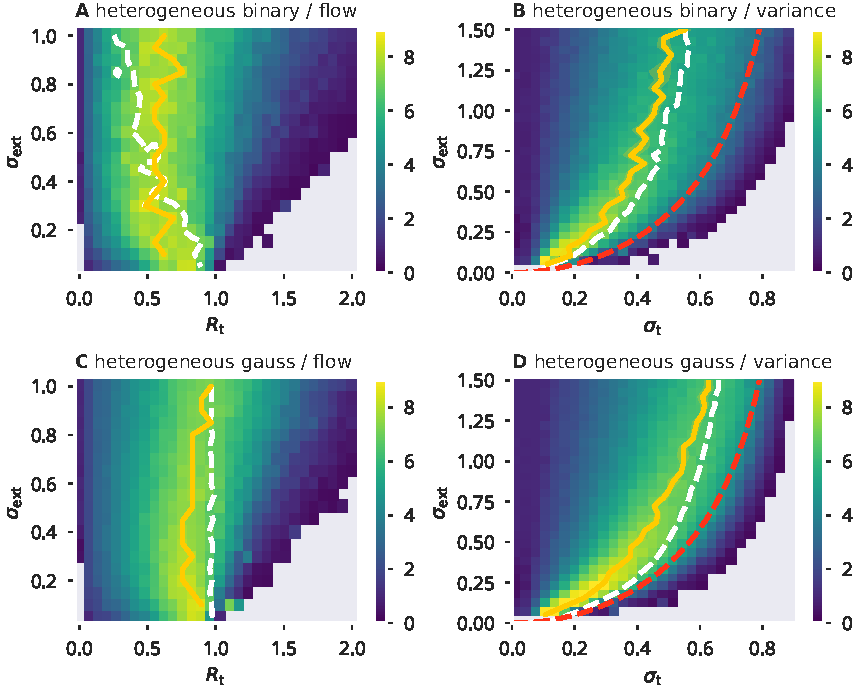
\includegraphics[width=5.78in]{./performance_sweep_composite.pdf}
    \label{fig:xor_perf_sweep}
    \caption{ Network performance as defined in (..) for different input types and after adaptation. For the cases where homogeneous/heterogeneous independent Gaussian input was used, the performance was tested with homogeneous/heterogeneous binary input with the same standard deviation $\sigma_{\rm ext}$. Yellow line marks optimal performance for a given $\sigma_{\rm ext}$. White dashed line corresponds to $R_{\rm a} = 1$. Red dashed line is the theoretical curve given by equation (..) (the solution $\sigma_{\rm ext} = \sigma_{\rm ext}(\sigma_{\rm t})$ of the Gaussian approximation for homogeneous input, without further simplifications). Performance that was lower than $0.2$ was masked in the colormap. Each grid point was averaged over five runs.
    {\bf A}: Homogeneous independent gaussian input.
     {\bf B}: Homogeneous identical binary input. 
     {\bf C}: Heterogeneous independent gaussian input. 
     {\bf D}: Heterogeneous identical binary input.}
  \end{figure}
\end{document}